\documentclass{beamer}
\usetheme{yahoo}

\usepackage{algorithmic}
\usepackage{amsmath, amsthm, amssymb}

\newcommand{\h}{h}
\newcommand{\HK}{\mathcal{H}_K}
\newcommand{\f}{f}
\newcommand{\btheta}{g}
\newcommand{\bbartheta}{\boldsymbol{\bar{\theta}}}

\newcommand{\Risk}{\mathcal{R}}
\newcommand{\RiskLoss}{\mathcal{E}^{\ell}}
\newcommand{\Ltworho}{\mathcal{L}^2_{\rho_\fX}}
\newcommand{\Lonerho}{\mathcal{L}^1_{\rho_\fX}}
\newcommand{\frho}{f_\rho}
\newcommand{\flrho}{f^{\ell}_\rho}
\newcommand{\fcla}{f_c}
\newcommand{\fl}{f^{\ell}}
\newcommand{\flambda}{f_\lambda}

%\newcommand{\normK}[1]{\left\|{#1}\right\|_{\mathcal{H}_K}}
\newcommand{\normK}[1]{\left\|{#1}\right\|_K}
\newcommand{\normL}[1]{\left\|{#1}\right\|_{\Ltworho}}
\newcommand{\normLOne}[1]{\left\|{#1}\right\|_{\Lonerho}}

\newcommand{\bx}{\boldsymbol{x}}
\newcommand{\bX}{\boldsymbol{X}}
\newcommand{\bu}{\boldsymbol{u}}
\newcommand{\by}{\boldsymbol{y}}
\newcommand{\bY}{\boldsymbol{Y}}
\newcommand{\sY}{\mathcal{Y}}
\newcommand{\bhatY}{\boldsymbol{\hat{Y}}}
\newcommand{\bbary}{\boldsymbol{\bar{y}}}
\newcommand{\bbarv}{\boldsymbol{\bar{v}}}
\newcommand{\bz}{\boldsymbol{z}}
\newcommand{\bZ}{\boldsymbol{Z}}
\newcommand{\bphi}{\boldsymbol{\phi}}
\newcommand{\bbarphi}{\boldsymbol{\bar{\phi}}}
\newcommand{\bbaru}{\boldsymbol{\bar{u}}}
\newcommand{\bbarw}{\bar{f}}
\newcommand{\bbarZ}{\boldsymbol{\bar{Z}}}
\newcommand{\bbarz}{\boldsymbol{\bar{z}}}
\newcommand{\bhatZ}{\boldsymbol{\hat{Z}}}
\newcommand{\bhatz}{\boldsymbol{\hat{z}}}
\newcommand{\barz}{\bar{z}}
\newcommand{\bS}{\boldsymbol{S}}
\newcommand{\bbarS}{\boldsymbol{\bar{S}}}
\newcommand{\bc}{\boldsymbol{c}}
\newcommand{\ba}{\boldsymbol{a}}
\newcommand{\bw}{\boldsymbol{w}}
\newcommand{\bW}{\boldsymbol{W}}
\newcommand{\bU}{\boldsymbol{U}}
\newcommand{\bv}{\boldsymbol{v}}
\newcommand{\bzero}{\boldsymbol{0}}
\newcommand{\balpha}{\boldsymbol{\alpha}}
\newcommand{\sA}{\mathcal{A}}
\newcommand{\sC}{\mathcal{C}}
\newcommand{\sX}{\mathcal{X}}
\newcommand{\sS}{\mathcal{S}}
\newcommand{\sZ}{\mathcal{Z}}
\newcommand{\sbarZ}{\bar{\mathcal{Z}}}
\newcommand{\fbag}{\bold{F}}


\DeclareMathOperator*{\argmin}{arg\,min}
%\newcommand{\argmax}[1]{\underset{#1}{\operatorname{argmax}}}

\newcommand{\todo}[1]{\textcolor{red}{TODO: #1}}
\newcommand{\fixme}[1]{\textcolor{red}{FIXME: #1}}

\newcommand{\field}[1]{\mathbb{#1}}
\newcommand{\fY}{\field{Y}}
\newcommand{\fX}{\field{X}}
\newcommand{\fH}{\field{H}}

\newcommand{\R}{\field{R}}
\newcommand{\Nat}{\field{N}}
\newcommand{\E}{\field{E}}



\newcommand\theset[2]{ \left\{ {#1} \,:\, {#2} \right\} }
\newcommand\inn[2]{ \left\langle {#1} \,,\, {#2} \right\rangle }
\newcommand\RE[2]{ D\left({#1} \| {#2}\right) }
\newcommand\Ind[1]{ \left\{{#1}\right\} }
\newcommand{\norm}[1]{\left\|{#1}\right\|}
\newcommand{\diag}[1]{\mbox{\rm diag}\!\left\{{#1}\right\}}

\newcommand{\defeq}{\stackrel{\rm def}{=}}
\newcommand{\sgn}{\mbox{\sc sgn}}
\newcommand{\scI}{\mathcal{I}}
\newcommand{\scO}{\mathcal{O}}

\newcommand{\dt}{\displaystyle}
\renewcommand{\ss}{\subseteq}
\newcommand{\wh}{\widehat}
\newcommand{\ve}{\varepsilon}
\newcommand{\hlambda}{\wh{\lambda}}
\newcommand{\yhat}{\wh{y}}

\newcommand{\hDelta}{\wh{\Delta}}
\newcommand{\hdelta}{\wh{\delta}}
\newcommand{\spin}{\{-1,+1\}}

%\newcommand{\theHalgorithm}{\arabic{algorithm}}

% \newtheorem{lemma}{Lemma}
% \newtheorem{theorem}{Theorem}
% \newtheorem{cor}{Corollary}
% \newtheorem{remark}{Remark}
% \newtheorem{prop}{Proposition}

\newcommand{\reals}{\mathbb{R}}
\newcommand{\sign}{{\rm sign}}

\newcommand{\eg}{e.g.}
\newcommand{\ie}{i.e.}
\newcommand{\etal}{et al.}

\renewcommand{\P}{{\bf{P}}}

\newcommand{\textc}{\color{blue}}
\newcommand{\fgc}{\color{red}}
\newcommand{\othc}{\color{green}}
\newcommand{\bgc}{\color{black}}
\newcommand{\titc}{\bf\fgc}

\newcommand{\hY}{\widehat {Y}}
\newcommand{\hp}{\widehat {p}}

\newcommand{\sfrac}[2]{\mbox{$\frac{#1}{#2}$}}

\DeclareMathOperator*{\Exp}{\mathbf{E}}
\DeclareMathOperator{\Wealth}{Wealth}
\newcommand{\grad}{\nabla}
\renewcommand{\H}{\mathcal{H}}  % Hilbert space
\DeclareMathOperator{\Regret}{Regret}
\DeclareMathOperator{\polylog}{polylog}
\DeclareMathOperator{\Reward}{Reward}


\usepackage[english]{babel}
% or whatever

%\usepackage[latin1]{inputenc}
\usepackage[utf8]{inputenc}   % replace by the encoding you are using
% or whatever

\usepackage{times}
\usepackage[T1]{fontenc}
% Or whatever. Note that the encoding and the font should match. If T1
% does not look nice, try deleting the line with the fontenc.


\title{Parameter-Free Convex Learning through Coin Betting}

\author{Francesco Orabona \and D\'avid P\'al}

\institute[] % (optional, but mostly needed)
{
Yahoo Research, New York
}

\date[June 24, 2016]{June 24, 2016}


%\beamerdefaultoverlayspecification{<+->}
\setbeamercovered{invisible}

\begin{document}

\titleframe{Parameter-Free Convex Learning through Coin Betting}{Francesco Orabona and D\'avid P\'al}{Yahoo Research, NY}
%
%
\begin{frame}{Are You Still Tuning/Learning/Adapting Hyperparameters?}
	Standard Machine Learning procedures
	
	\vspace{1cm}
	
	Regularized empirical risk minimization:
	\[
	\argmin_{w \in \R^d} \ \frac{\lambda}{2} \norm{w}^2 + \sum_{i=1}^N f(w, x_i, y_i)
	\]
	where $f$ is convex in $w$.
	\begin{itemize}
	\item<2> How do you choose the regularizer weight $\lambda$?
	\end{itemize}
\end{frame}
%
%
\begin{frame}{Are You Still Tuning/Learning/Adapting Hyperparameters?}
	Standard Machine Learning procedures
	
	\vspace{1cm}
	
	Stochastic approximation:
	\[
	w_t = w_{t-1} - \eta_t \grad f(w_{t-1}, x_t, y_t)
	\]
	where $f$ is convex in $w$.
	\begin{itemize}
	\item<2> How do you choose the learning rate $\eta_t$?
	\end{itemize}
\end{frame}
%
%
\begin{frame}{Wasn't machine learning about learning \emph{automatically} from data?}

\begin{itemize}
\item There is a history of 7 years of parameter-free algorithms that \emph{do not have learning rates nor regularizers to tune}.
\item But they were very unintuitive and complex
\end{itemize}
\end{frame}
%
%
\begin{frame}{One Coin to Rule Them All}


\makebox[\linewidth][c]{
\begin{columns}[c]
  \begin{column}{3cm}
    \begin{figure}
      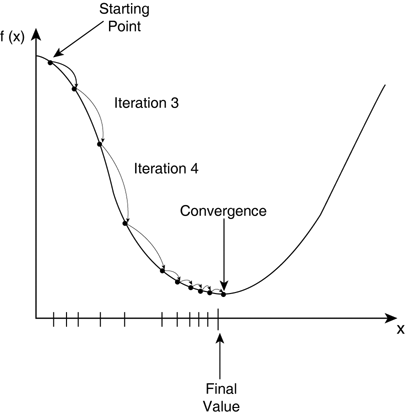
\includegraphics[width=4cm]{../poster/figs/gd}
    \end{figure}
  \end{column}
  \begin{column}{5cm}
  \center
  \huge
  is equivalent to
  \end{column}
  \begin{column}{4cm}
    \begin{figure}
      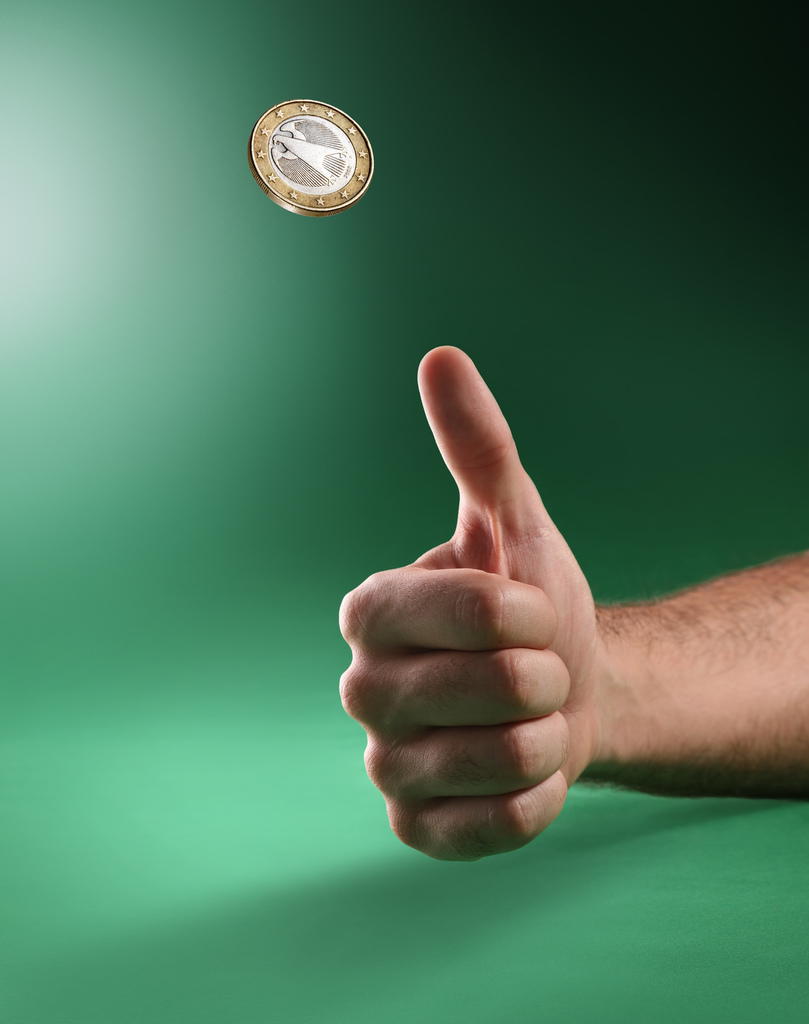
\includegraphics[width=3cm]{../poster/figs/coin_toss}
    \end{figure}
  \end{column}
\end{columns}
}


\center
Online Coin betting algorithms give rise to \emph{optimal} and \emph{parameter-free} learning algorithms

\end{frame}
%
%


\begin{frame}{Simple Algorithm \& Good Results}

\begin{columns}[c]
  \begin{column}{5cm}
   \small 
   \begin{itemize}
    \item Parameter-free
    \item Extremely simple algorithm
    \item Same complexity of SGD
    \item Kernelizable
    \end{itemize}
  \end{column}
  \begin{column}{6cm}
    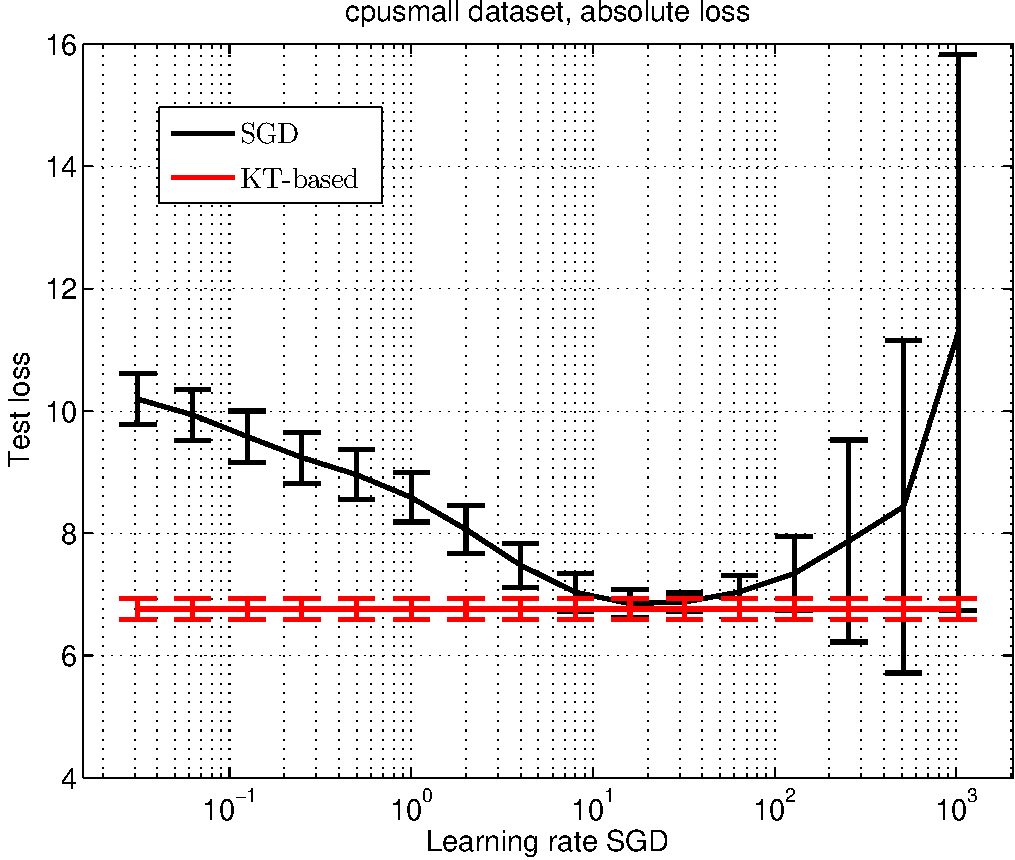
\includegraphics[width=0.9\textwidth]{../figs/cpusmall_kt_train_test-crop}
  \end{column}
\end{columns}

\vspace{.25cm}

%\begin{theorem}
%For any sequence of Lipschitz convex losses
%Define $n(\bx):=\max(\|\bx\|,\|\bx\|^2)$ and set $H_t=\sum_{i=1}^t L^2 n(\bx_t)+ \delta$, $\alpha_t = a \sqrt{H_{t}}$, $\beta_t = (H_{t})^\frac{3}{2}$, where $\delta\geq0$. Set in OMD $f_t(\bw)=\alpha_t \|\bw\| \left(\ln \left(\beta_t \|\bw\| \right)-1\right)$, and $\bz_t=-\ell'_t(\bw_t^\top\bx_t) \bx_t$.
%\[
%Regret(T) \leq \scO\left(\|\bu\| \sqrt{T} \left(\ln \left( T^{1.5} \|\bu\| \right)-1\right) \right)
%\]
%\end{theorem}

\begin{center}
\huge
See how at the poster!
\end{center}

\end{frame}

\end{document}

